\documentclass[10.5pt]{config}

\major{生物医学工程}
\name{卢星余}
\partner{} % 签名栏
% \title{}
\stuid{3220100425}
\date{2025年3月13日}
\lab{教6-204}
\course{生物医学图像处理}
\instructor{吴丹}
\grades{}
\expname{lab2} % 实验名字
\exptype{} % 实验类型

\begin{document}

% \maketitlepage % 封面
% \maketoc % 目录
\makeheader % 首页头部


\section{实验目的和要求}
了解并实现基本的医学图像空间变换和强度变换;掌握直方图均衡化的原理和实现方法;学习如何加载和处理CT和MRI图像数据。

\section{实验内容和原理}
\subsection{预实验:加载医学图像数据}
\begin{itemize}
    \item 将lab2\_CT.npy和lab2\_MRI.npy数据加载到数组中
    \item 显示医学图像
\end{itemize}

\subsection{Project1:空间变换}
\begin{itemize}
    \item 使用提供的脑部MRI数据,设计并实现以下仿射变换:
    \begin{itemize}
        \item 沿垂直方向平移
        \item 缩放至原尺寸的一半 (M/2, N/2)
        \item 沿x轴或y轴翻转
        \item 围绕原点旋转π/4
        \item 组合以上变换
    \end{itemize}
\end{itemize}

\subsection{Project2:强度变换}
\begin{itemize}
    \item 使用提供的CT数据,编写代码实现:
    \begin{itemize}
        \item 对数变换
        \item 幂变换
    \end{itemize}
    \item 调整参数以展示最佳视觉效果
    \item 解释不同方法之间的主要差异
    \item 说明参数选择的方法和理由
\end{itemize}

\subsection{Project3:直方图均衡化}
\begin{itemize}
    \item 使用提供的CT数据:
    \begin{itemize}
        \item 计算并显示灰度直方图
        \item 实现直方图均衡化
        \item 分析增强后图像的直方图变化
        \item 解释直方图均衡化带来的增强效果
    \end{itemize}
\end{itemize}

\section{实验设备及材料}
Python

\section{实验方法和步骤}
根据实验要求撰Python脚本运行
\subsection{预实验:加载医学图像数据}
\begin{enumerate}
    \item 使用NumPy加载.npy格式的医学图像数据
\end{enumerate}

\subsection{Project1:空间变换}
\begin{enumerate}
    \item 加载MRI图像数据
    \item 实现并测试各种仿射变换函数(平移、缩放、翻转、旋转)
    \item 设计组合变换
    \item 将原始图像与变换后的图像进行可视化比较
\end{enumerate}

\subsection{Project2:强度变换}
\begin{enumerate}
    \item 加载CT图像数据
    \item 实现对数变换函数,使用不同参数值测试
    \item 实现幂变换函数,使用不同参数值测试
    \item 设计评估指标比较不同参数设置的效果
    \item 分析并选择最佳参数配置
\end{enumerate}

\subsection{Project3:直方图均衡化}
\begin{enumerate}
    \item 加载CT图像数据
    \item 计算并显示原始图像的灰度直方图
    \item 实现直方图均衡化算法
    \item 对均衡化后的图像计算新的直方图
    \item 比较原始图像和均衡化后图像的差异
    \item 分析直方图变化与图像增强效果的关系
\end{enumerate}

\section{实验结果与分析}

\subsection{预实验:加载医学图像数据}
成功加载了CT和MRI医学图像数据。
\begin{figure}[!htbp]
    \centering
    \begin{minipage}[b]{0.45\linewidth}
        \centering
        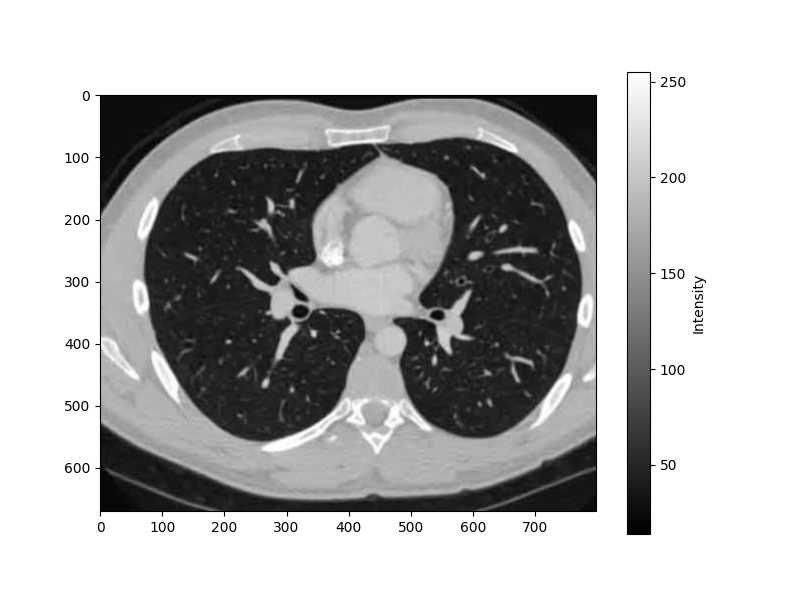
\includegraphics[width=1.0\textwidth]{figures/CT.png}
        \caption{CT.png}
    \end{minipage}%
    \begin{minipage}[b]{0.45\linewidth}
        \centering
        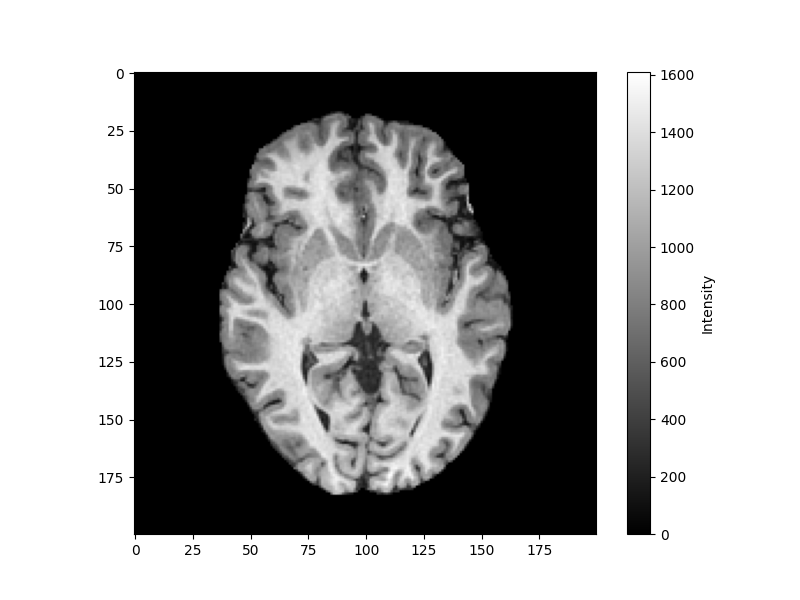
\includegraphics[width=1.0\textwidth]{figures/MRI.png}
        \caption{MRI.png}
    \end{minipage}
\end{figure}
\subsection{Project1:空间变换}
\begin{figure}[htbp]
    \centering
    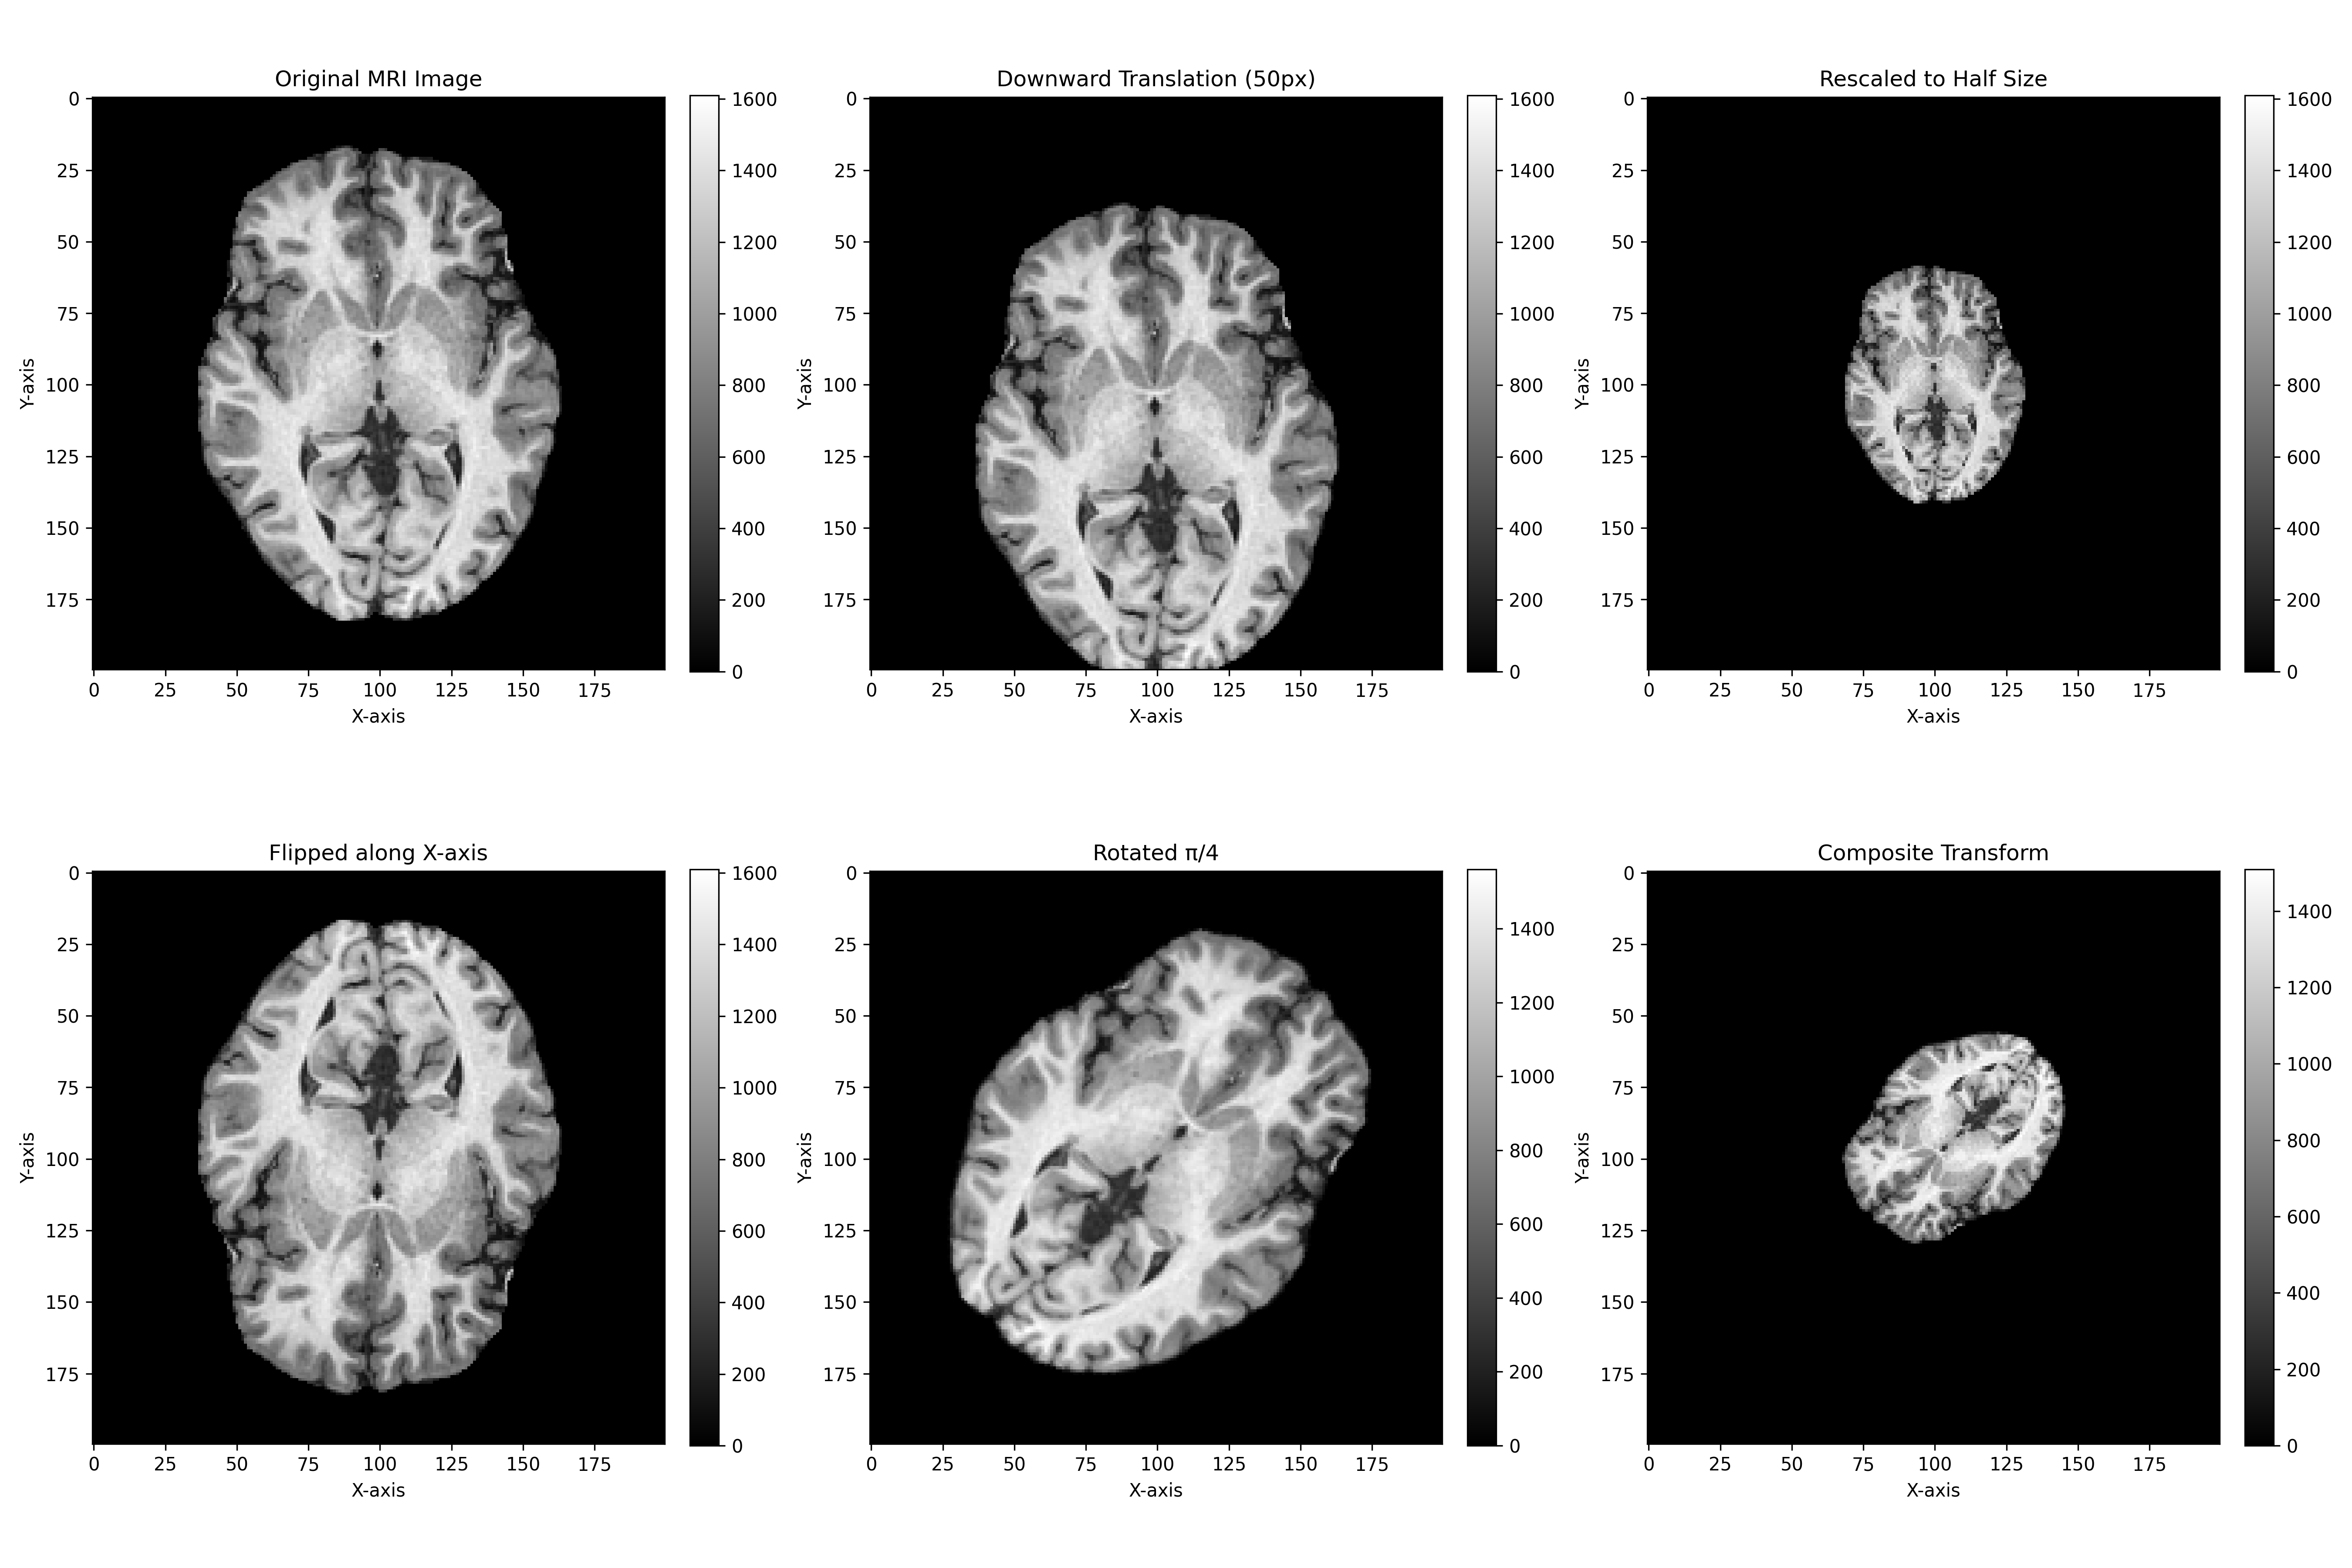
\includegraphics[width=1.0\linewidth]{figures/MRI_affine_transformations.png}
    \caption{MRI数据的仿射变换结果}
    \label{fig:mri_affine}
\end{figure}

如图\ref{fig:mri_affine}所示,我们对MRI图像实现了多种仿射变换。平移变换将图像沿垂直方向移动了约20像素;缩放变换将图像尺寸减小至原来的一半;翻转变换沿x轴实现了图像镜像;旋转变换使图像围绕原点旋转了pi/4弧度。最后,我们还设计了一个组合变换,包含了平移、旋转和缩放。通过这些变换,我们可以调整医学图像的位置和方向,以便更好地观察和分析。

\subsection{Project2:强度变换}
\begin{figure}[htbp]
    \centering
    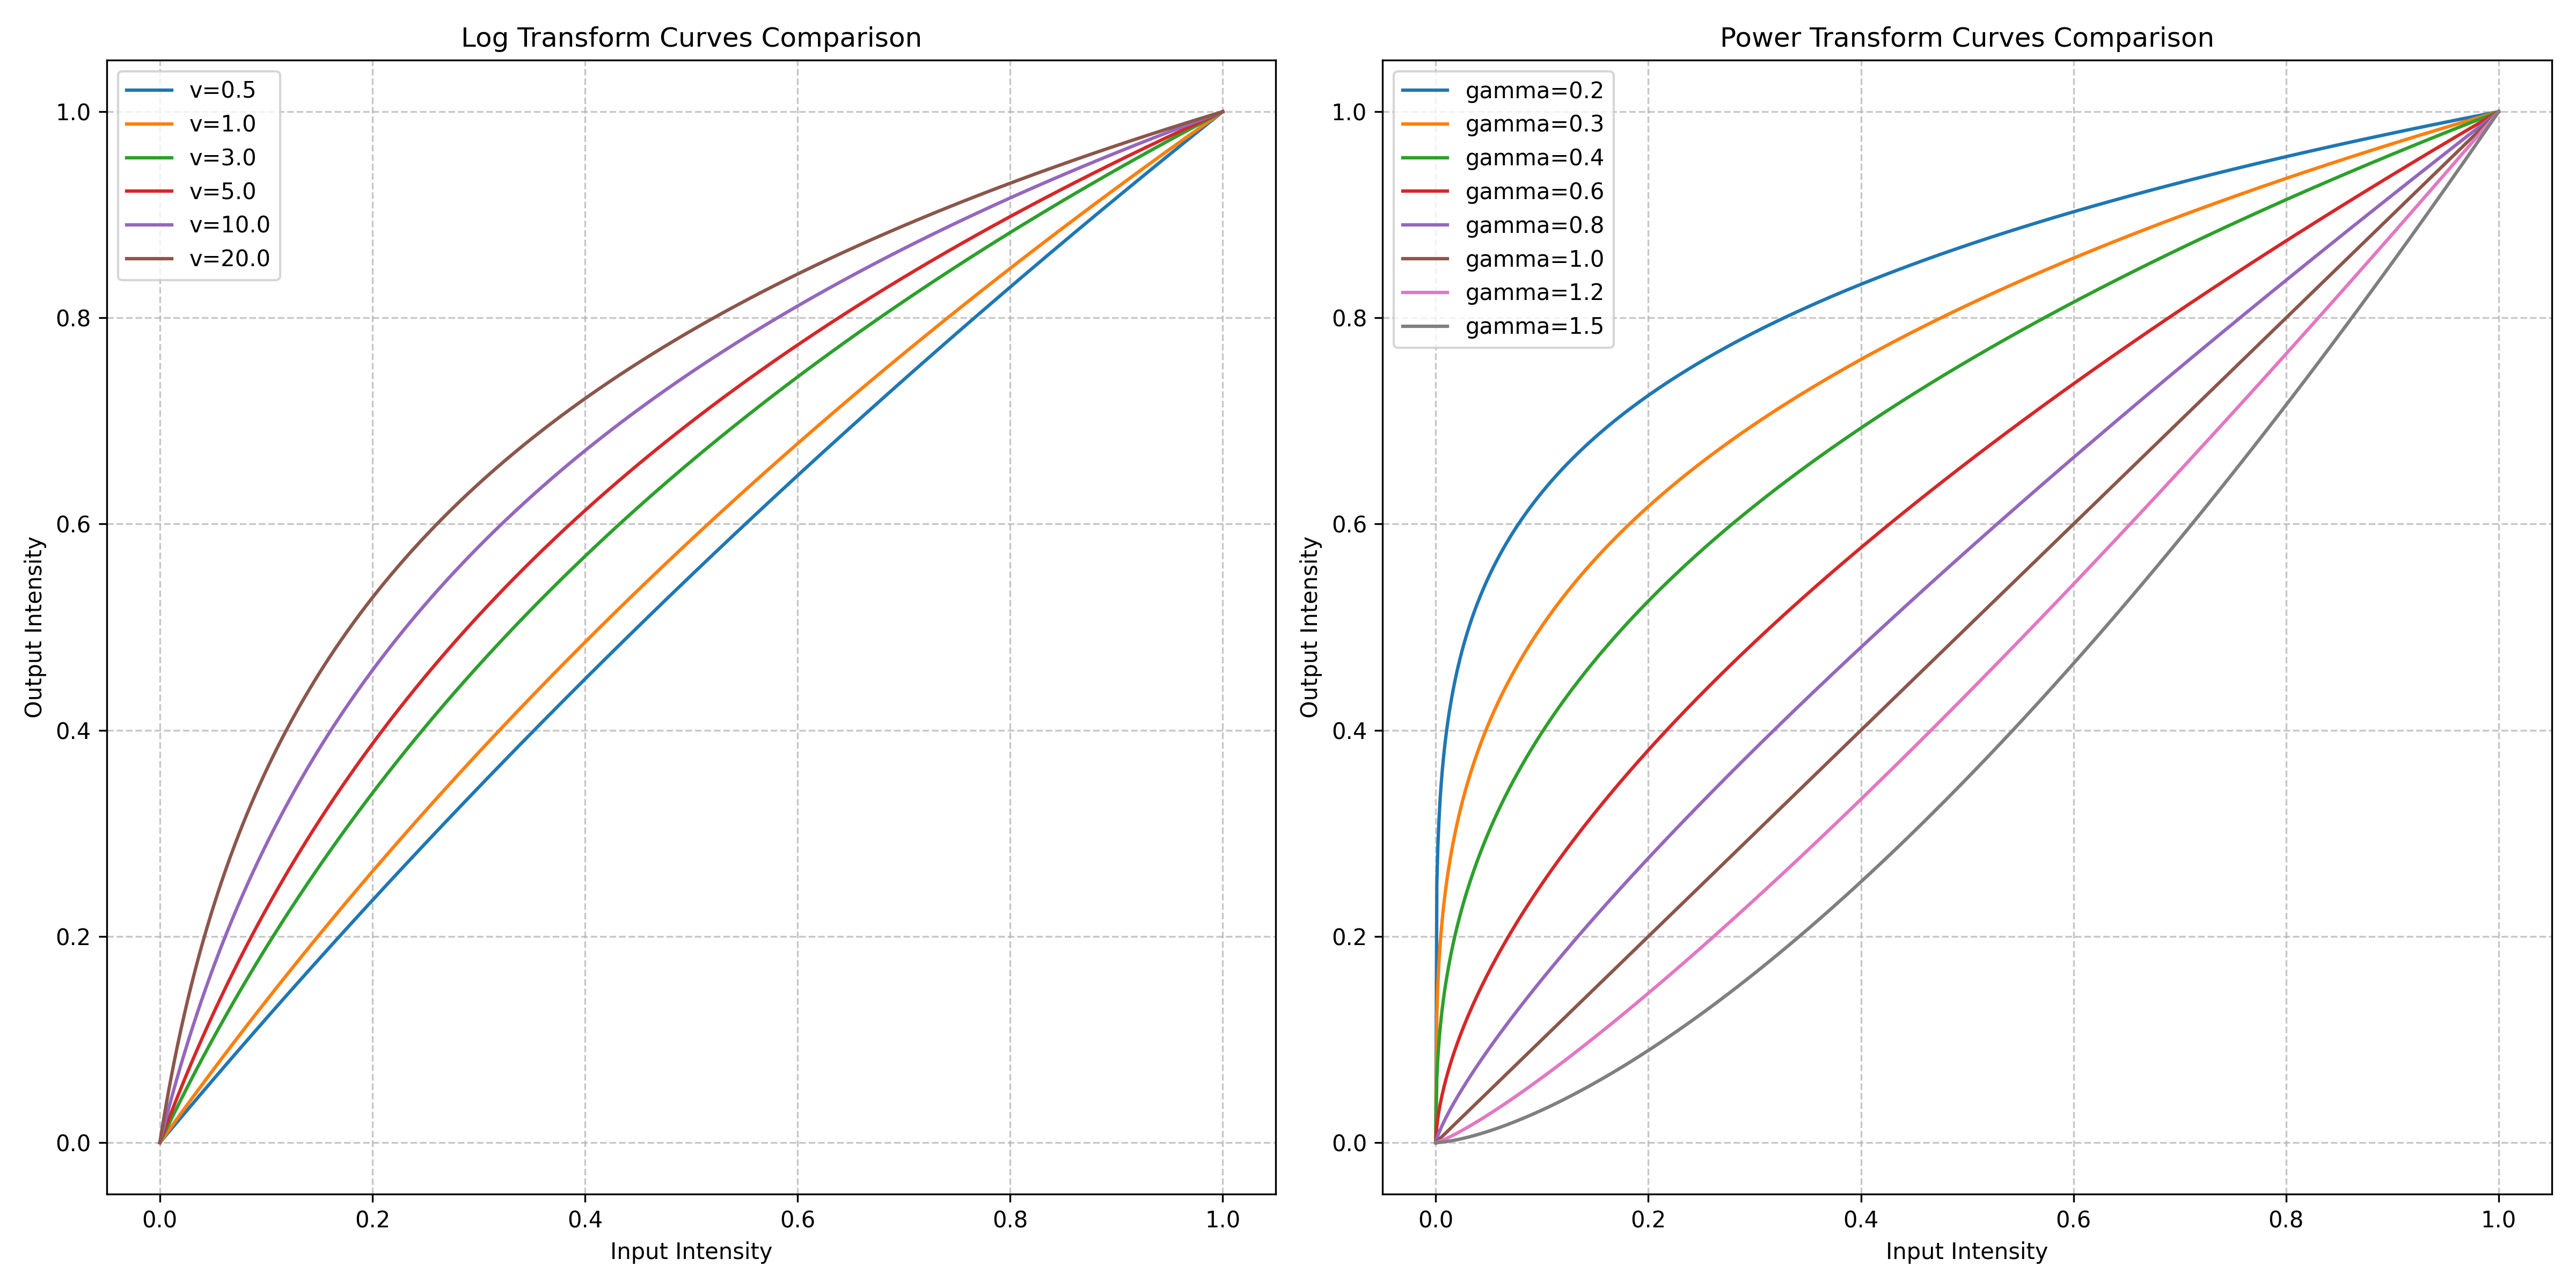
\includegraphics[width=1.0\linewidth]{figures/CT_transform_curves.png}
    \caption{对数变换和幂变换曲线比较}
    \label{fig:transform_curves}
\end{figure}

\begin{figure}[htbp]
    \centering
    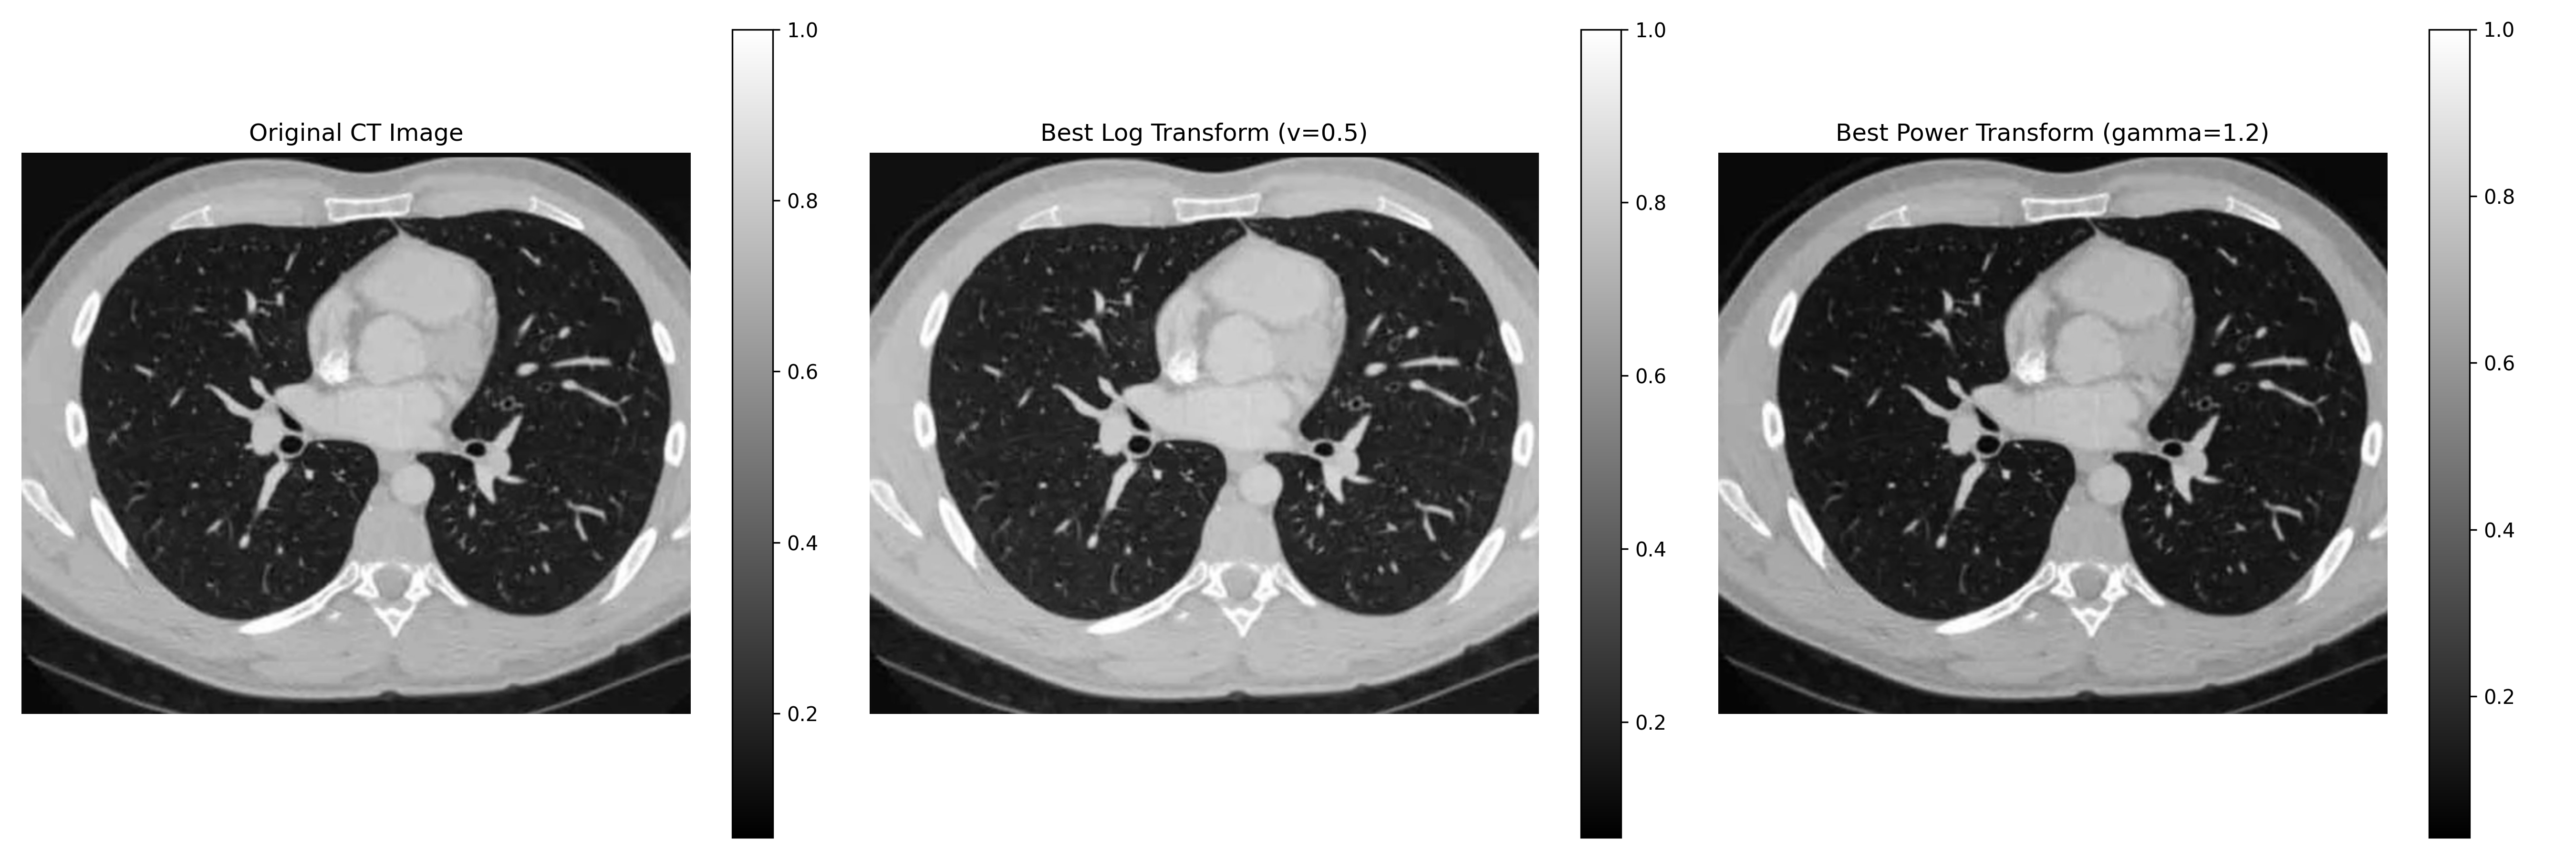
\includegraphics[width=1.0\linewidth]{figures/CT_best_transformations.png}
    \caption{原始CT图像与最佳对数变换和幂变换结果比较}
    \label{fig:best_transforms}
\end{figure}
\begin{figure}[htbp]
    \centering
    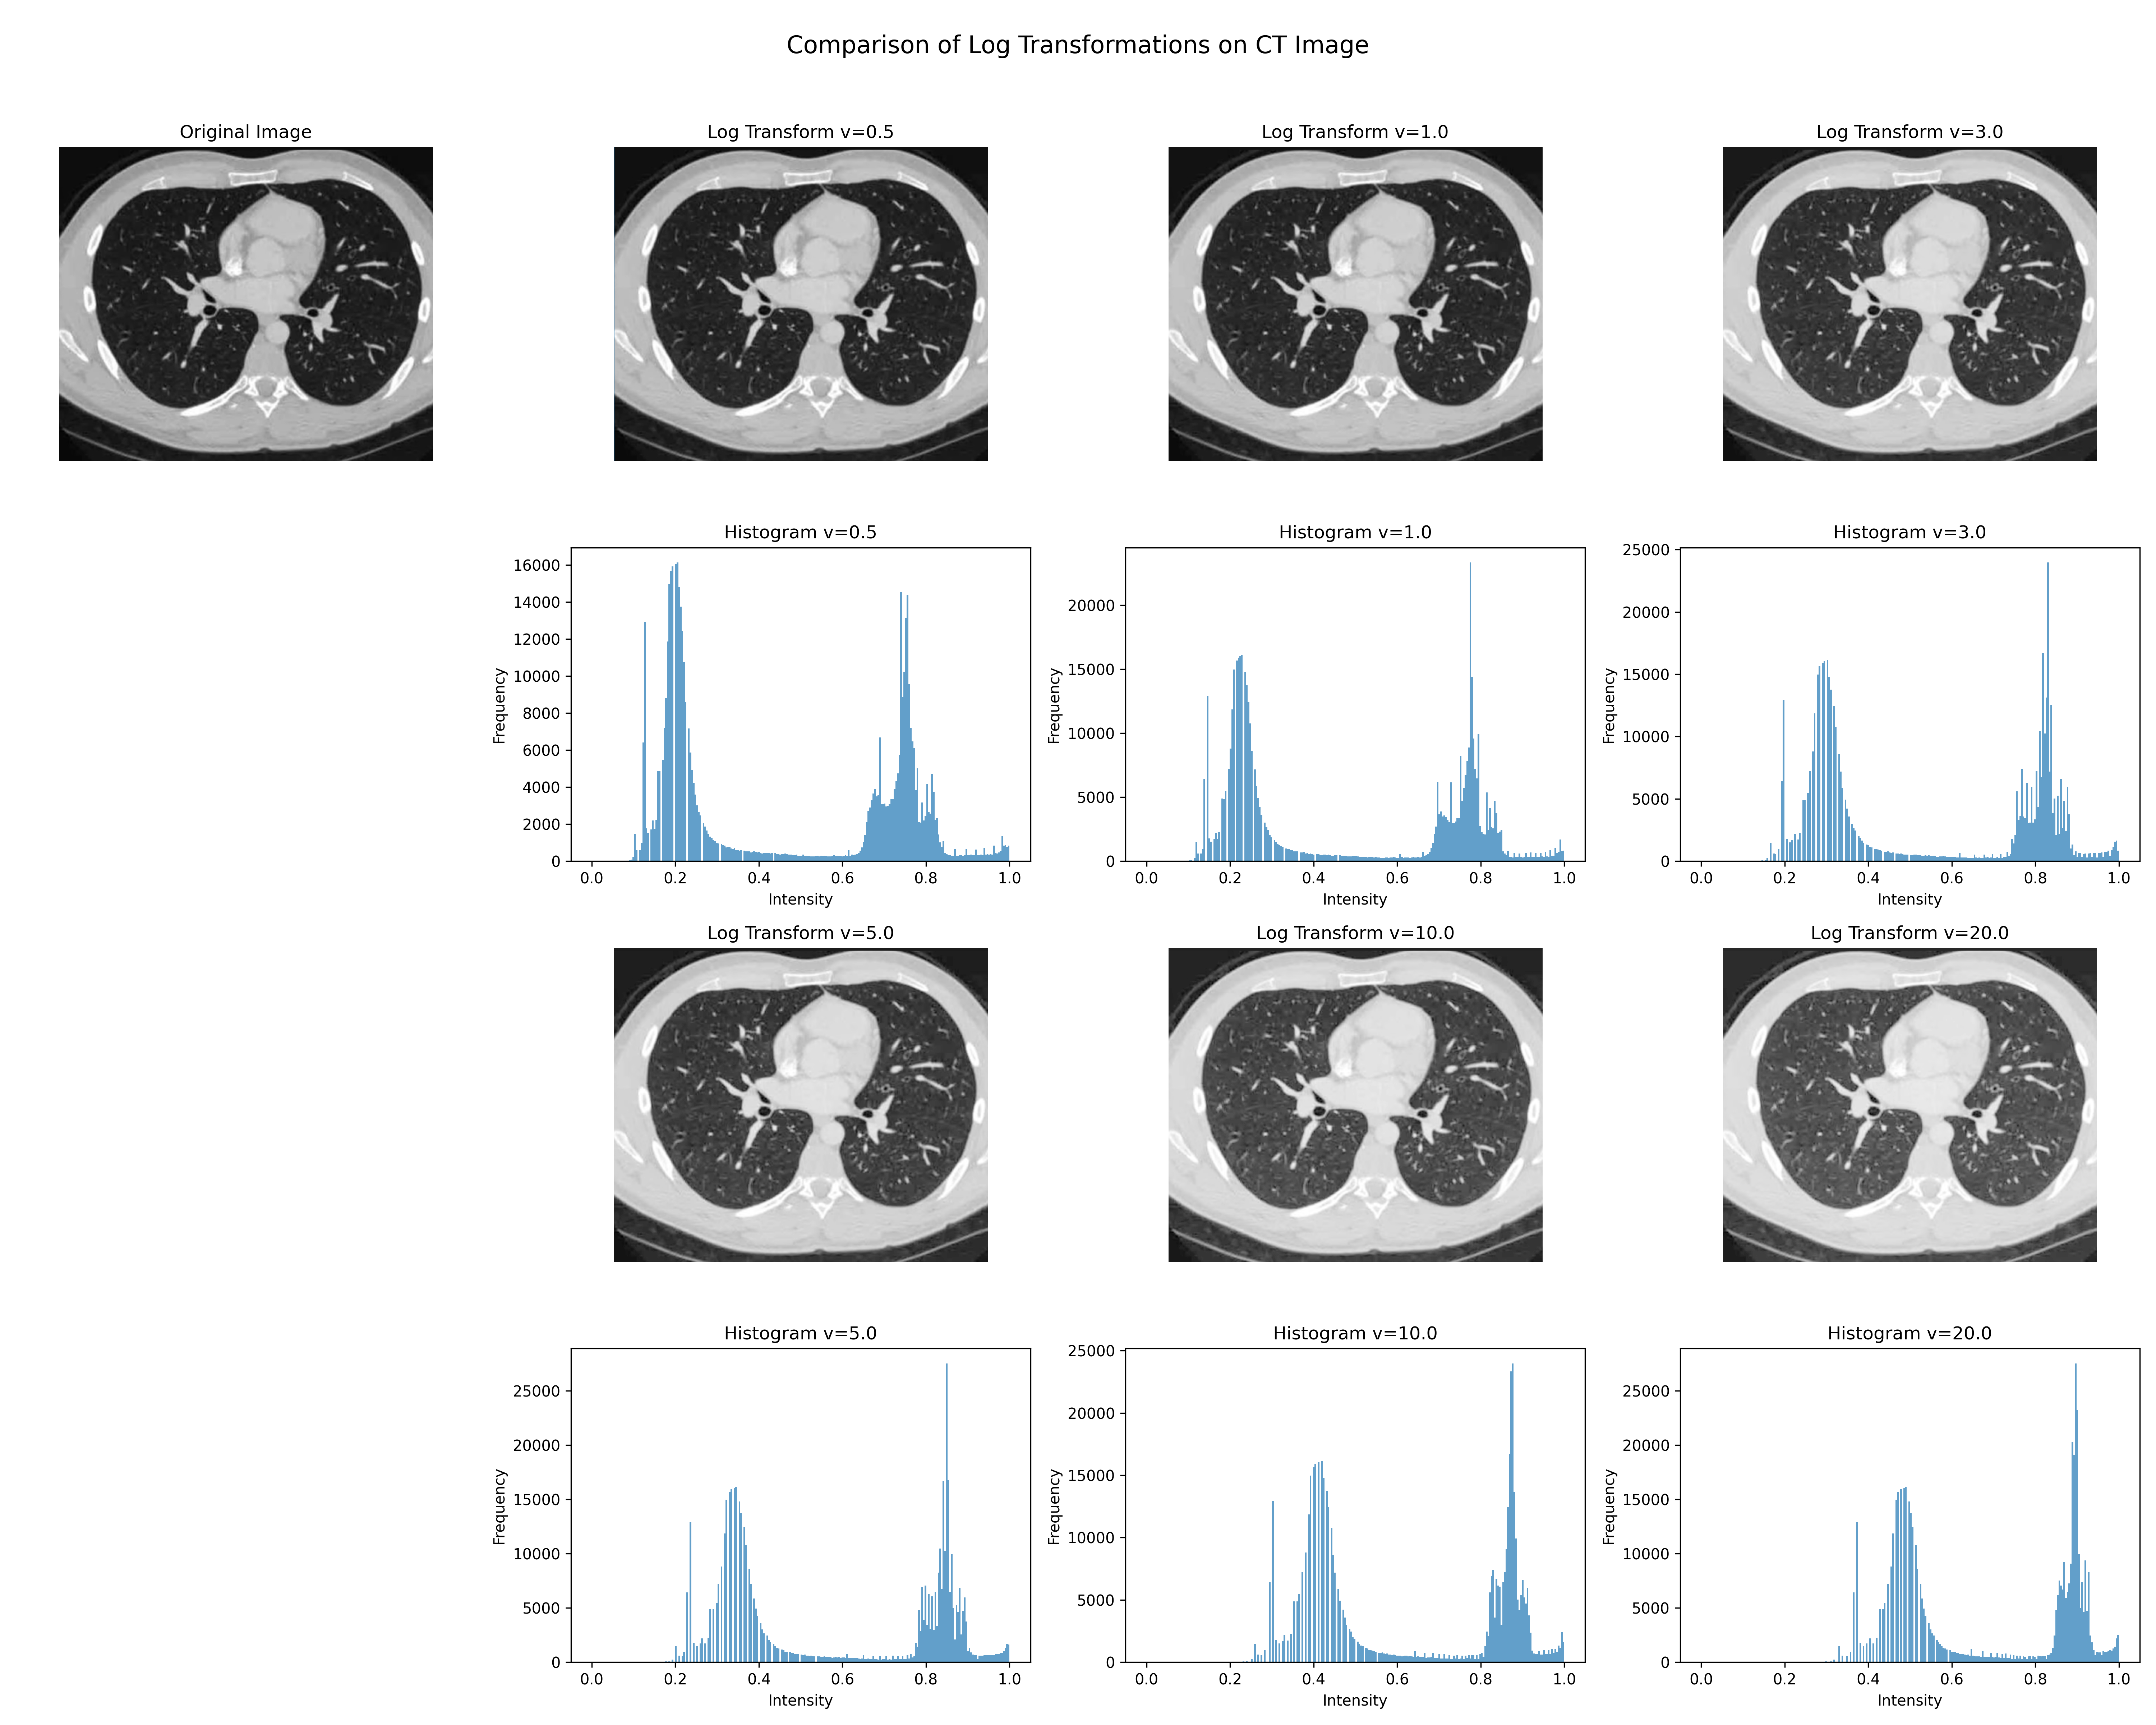
\includegraphics[width=1.0\linewidth]{figures/CT_log_transforms_comparison.png}
    \caption{原始CT图像与对数变换结果比较}
    \label{fig:log_transforms_comparison}
\end{figure}\begin{figure}[htbp]
    \centering
    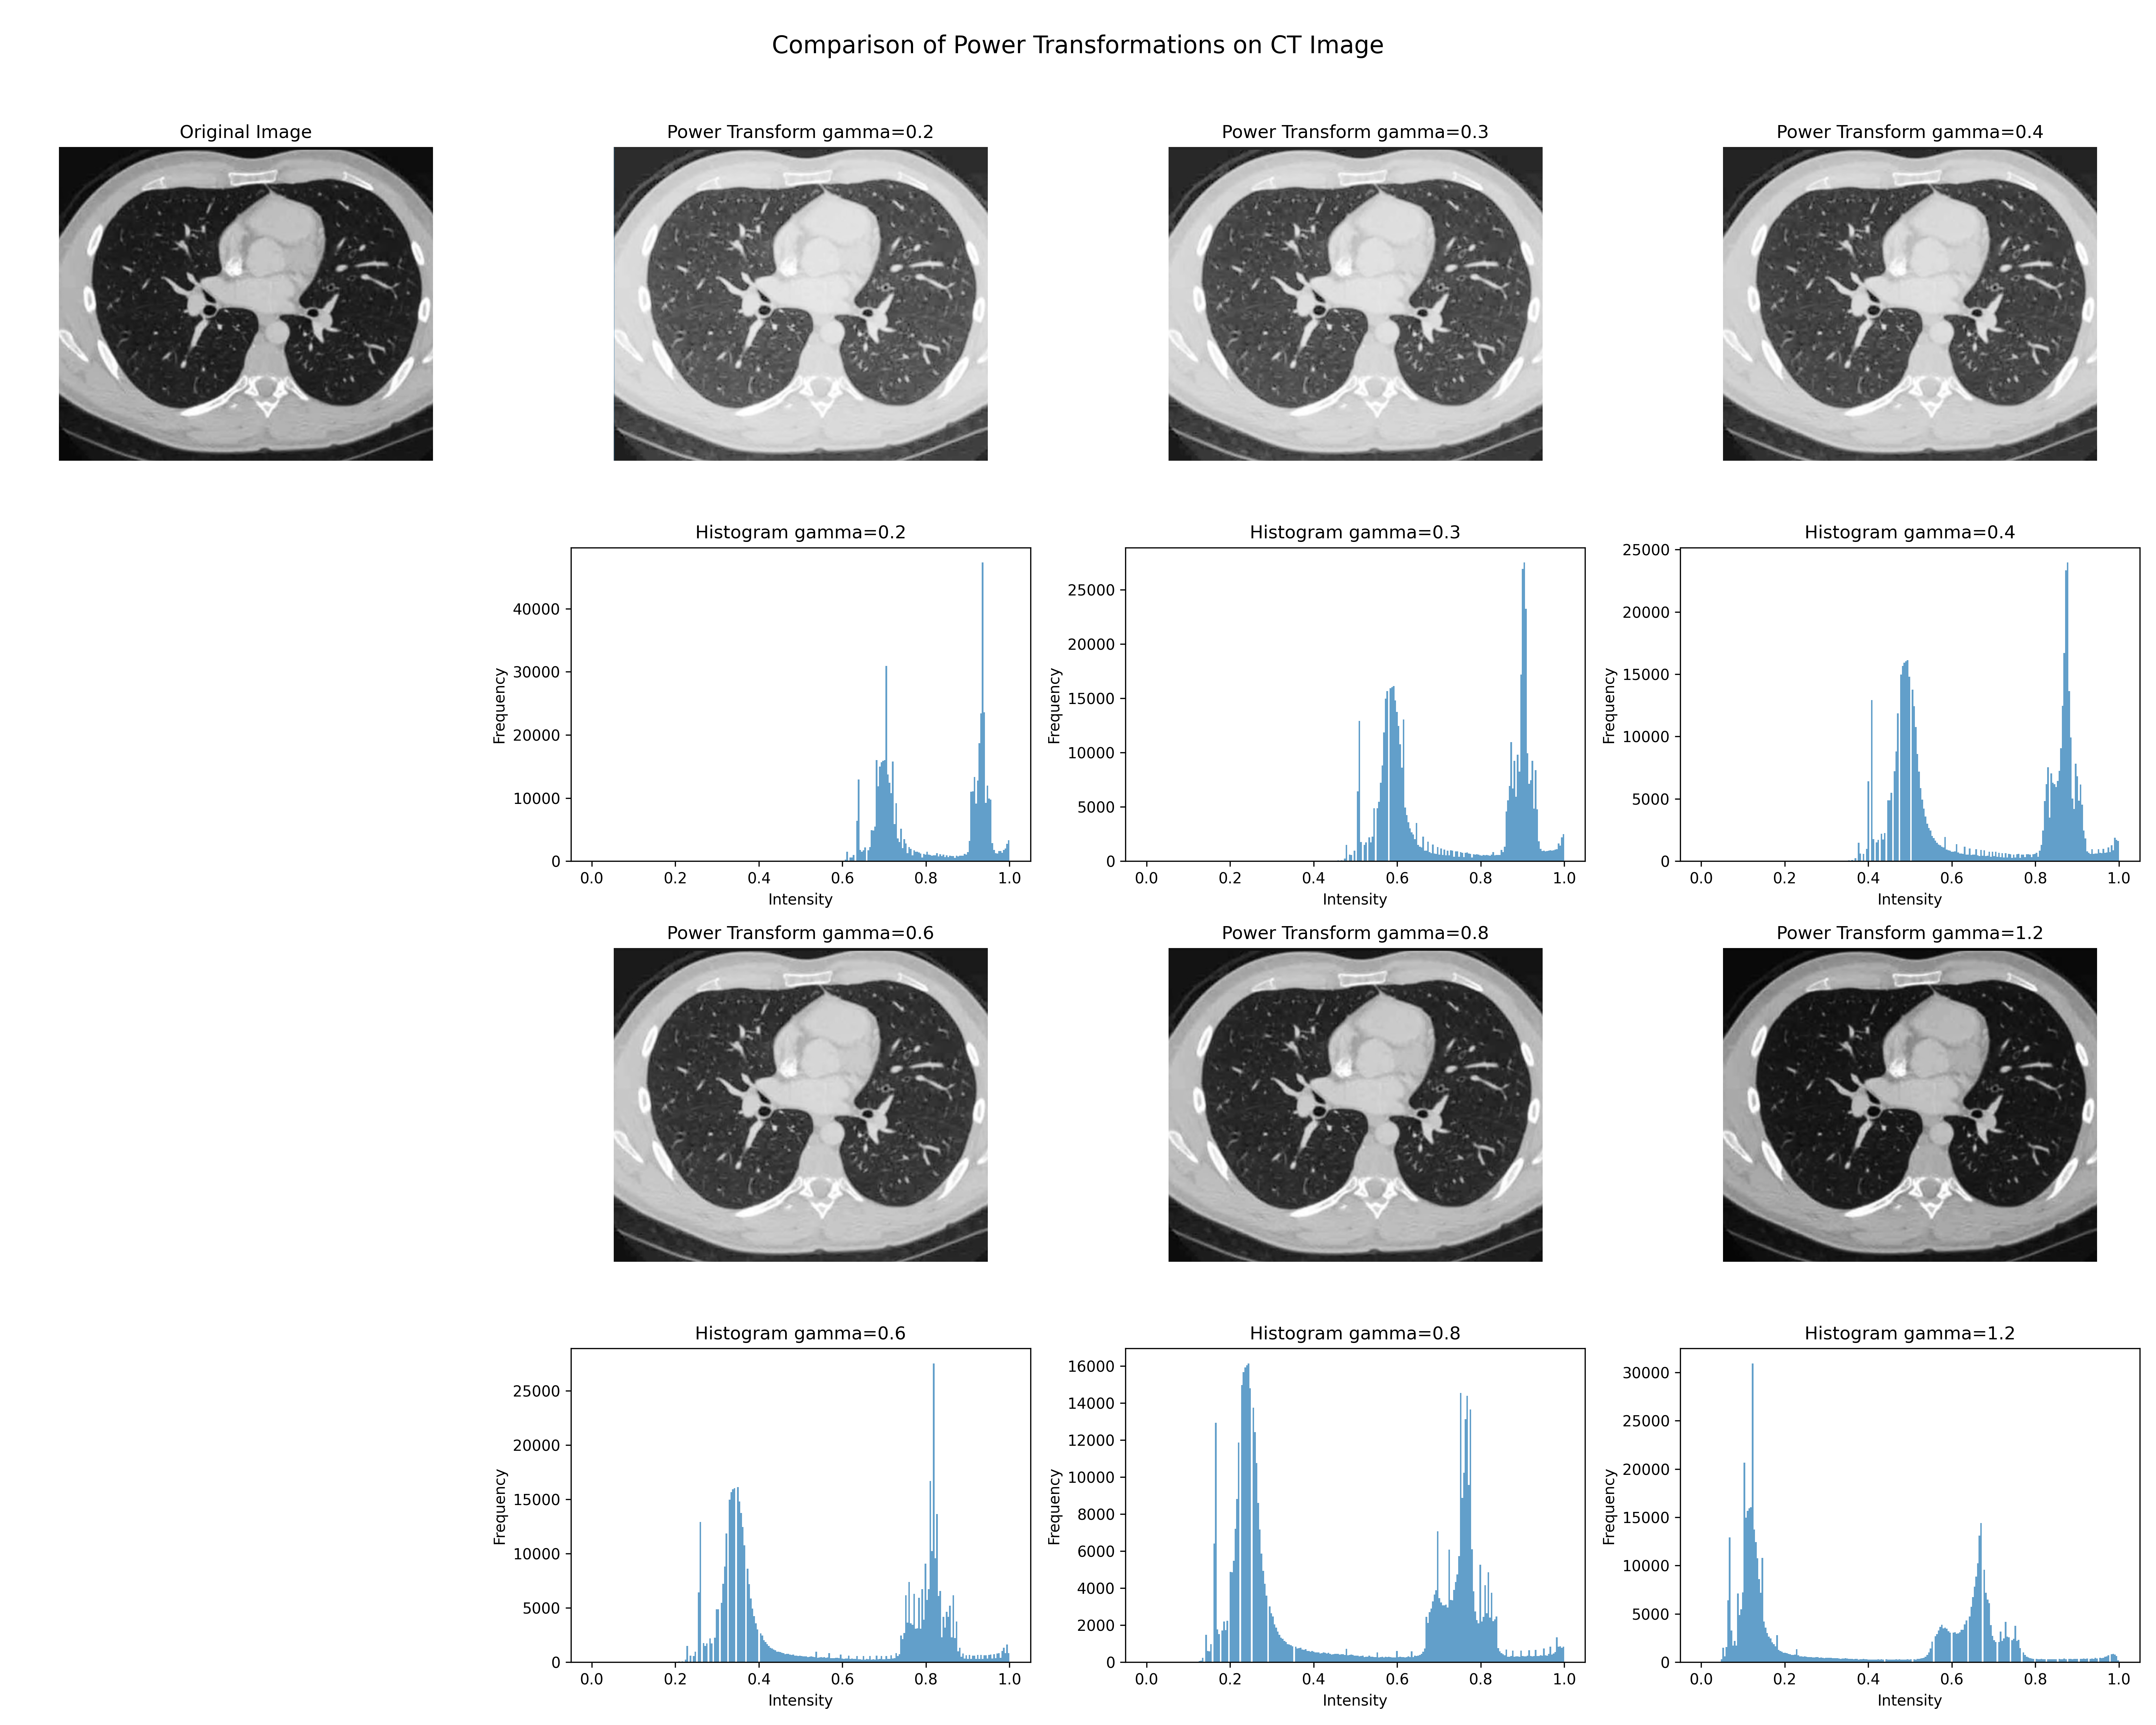
\includegraphics[width=1.0\linewidth]{figures/CT_power_transforms_comparison.png}
    \caption{原始CT图像与幂变换结果比较}
    \label{fig:power_transforms_comparison}
\end{figure}
图\ref{fig:transform_curves}展示了不同参数设置的对数变换和幂变换曲线。对数变换使用修正公式$s = c \cdot \log(1 + v \cdot r) / \log(1 + v)$,其中$v$控制非线性程度;幂变换使用公式$s = c \cdot r^{\gamma}$,其中$\gamma$控制曲线形状。
如图\ref{fig:log_transforms_comparison}和图\ref{fig:power_transforms_comparison}所示,我们对原始CT图像进行了对数变换和幂变换不同参数的比较。
如图\ref{fig:best_transforms}所示,我们通过调整参数找到了最佳的变换效果。对于对数变换,最佳参数为v=0.5;对于幂变换,最佳参数为gamma=1.2。这些参数是基于以下量化指标自动选择的:对比度比率、熵增益、结构相似性和边缘增强效果。

对数变换和幂变换的主要区别在于它们对不同强度区域的增强特性:
\begin{itemize}
    \item 对数变换在低强度区域提供更强的增强效果,但对高强度区域的区分度较低
    \item 幂变换(gamma < 1.5)可以更均匀地增强暗区域,同时保留更多的整体结构特征
    \item 对数变换的非线性程度随参数v变化更灵活,而幂变换在gamma接近0时会更快速地压缩高强度值
\end{itemize}
\begin{figure}[htbp]
    \centering
    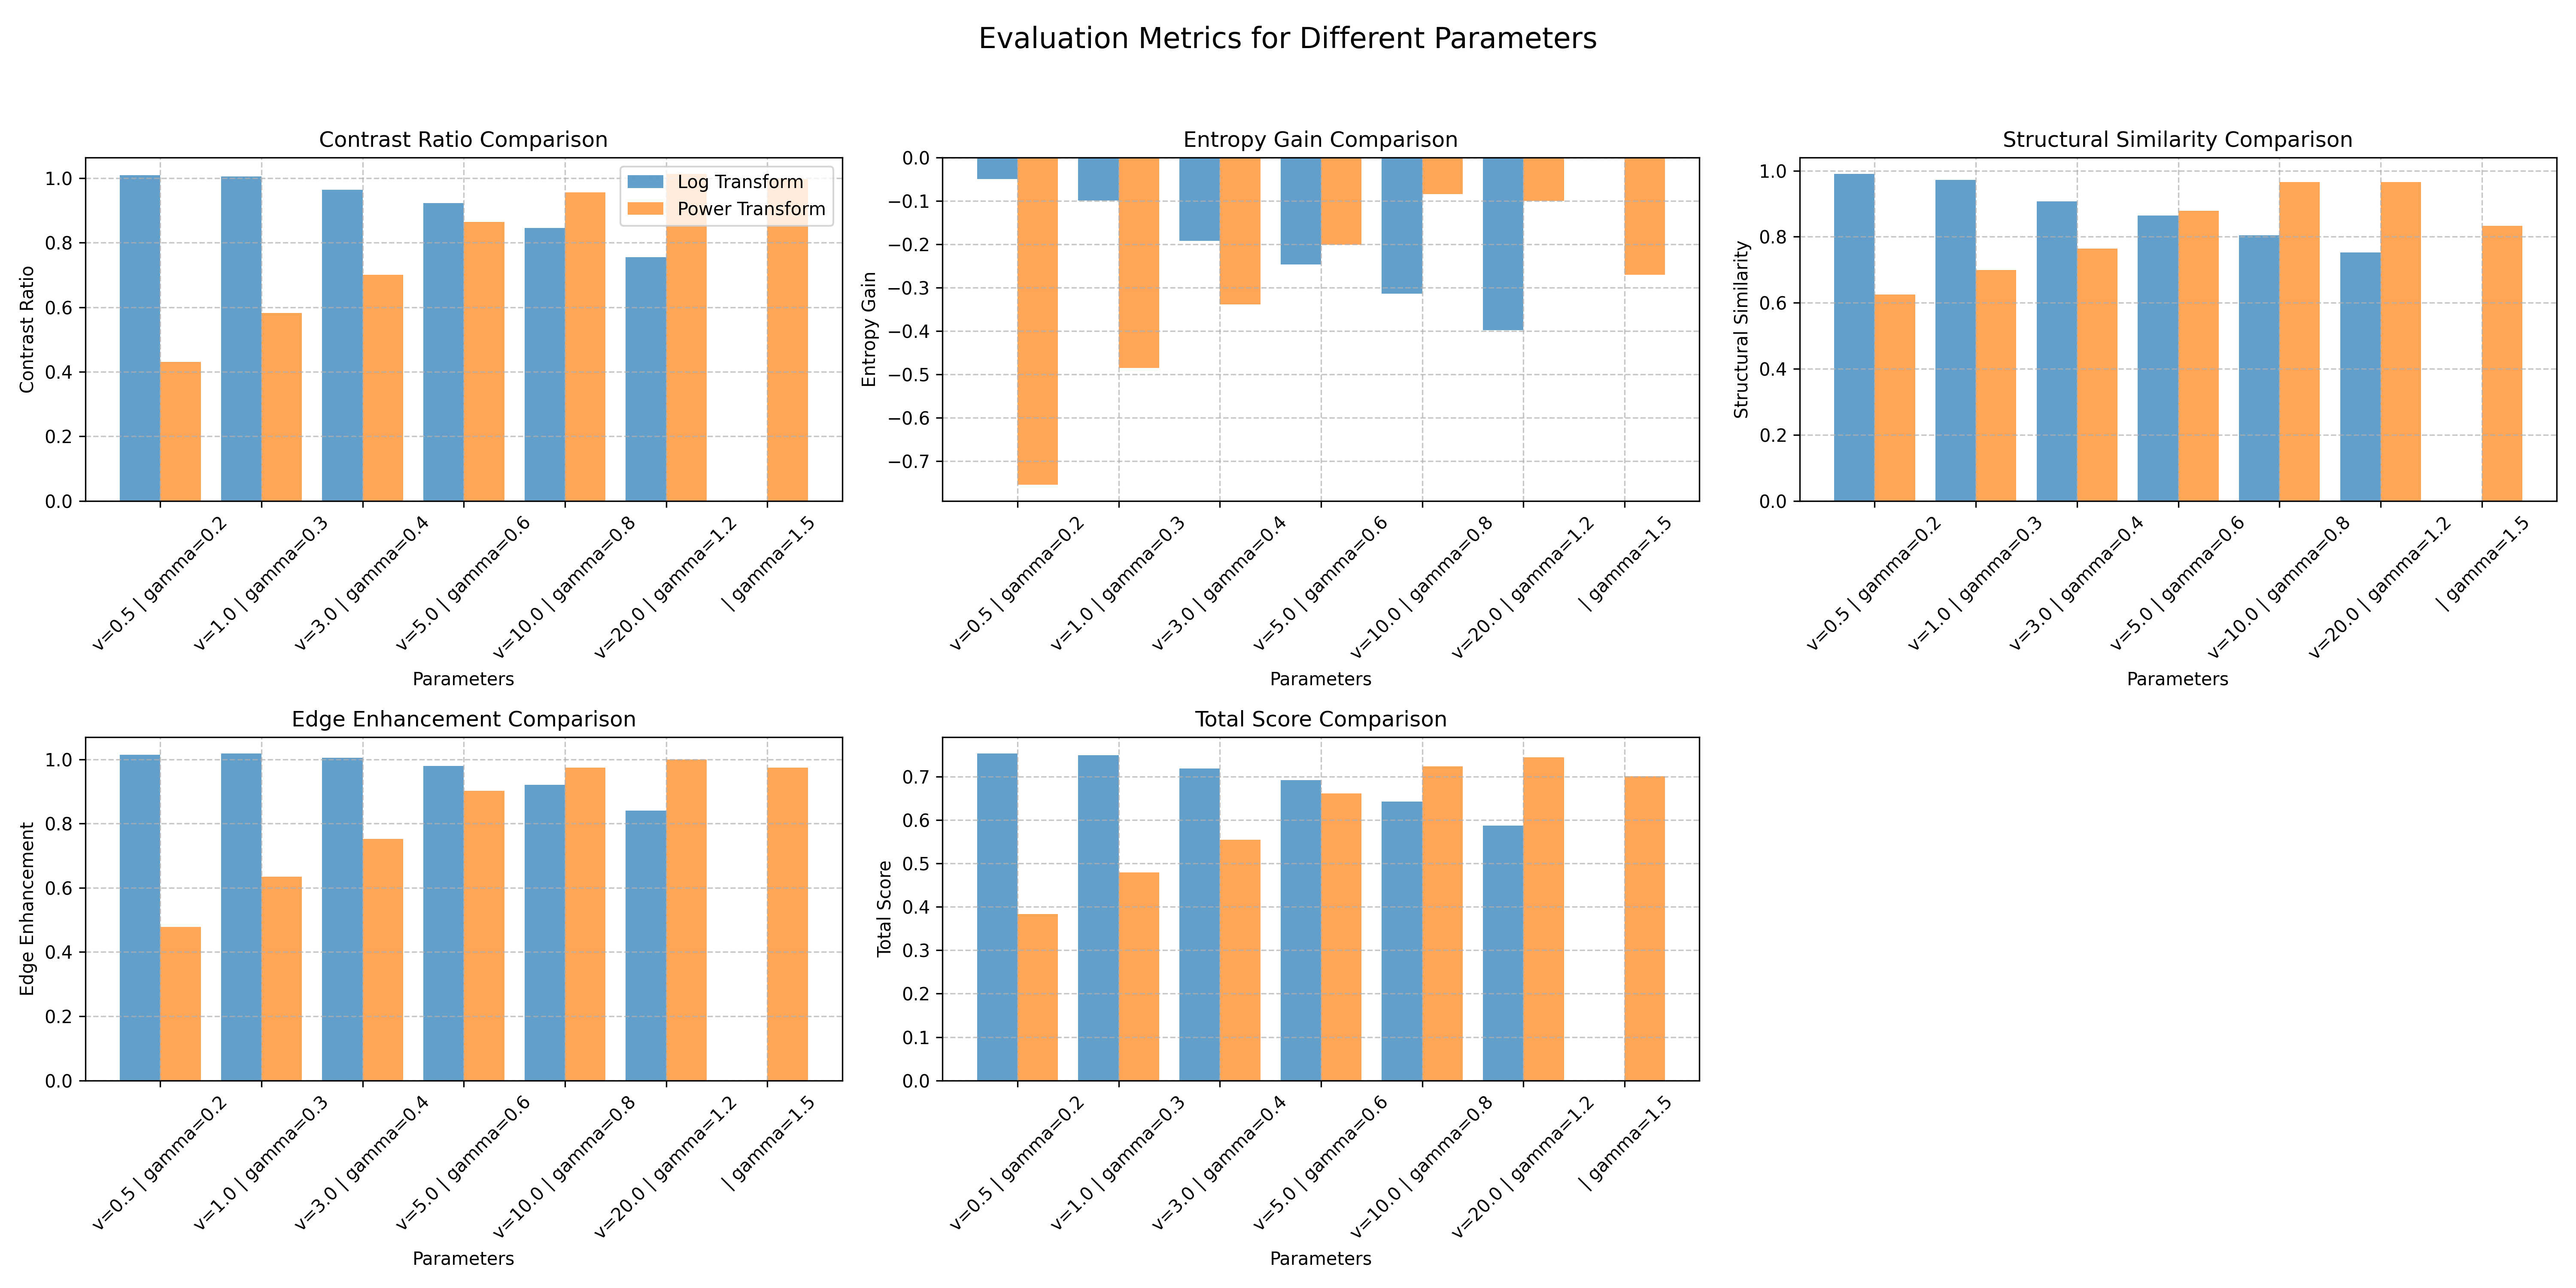
\includegraphics[width=1.0\linewidth]{figures/CT_transform_metrics.png}
    \caption{综合评分}
    \label{fig:metrics}
\end{figure}

如图\ref{fig:metrics}参数选择依据了多个客观评估指标的综合评分,包括:提高对比度的能力、信息增益量、图像原始结构保留程度以及边缘清晰度的提升。

\subsection{Project3:直方图均衡化}
\begin{figure}[htbp]
    \centering
    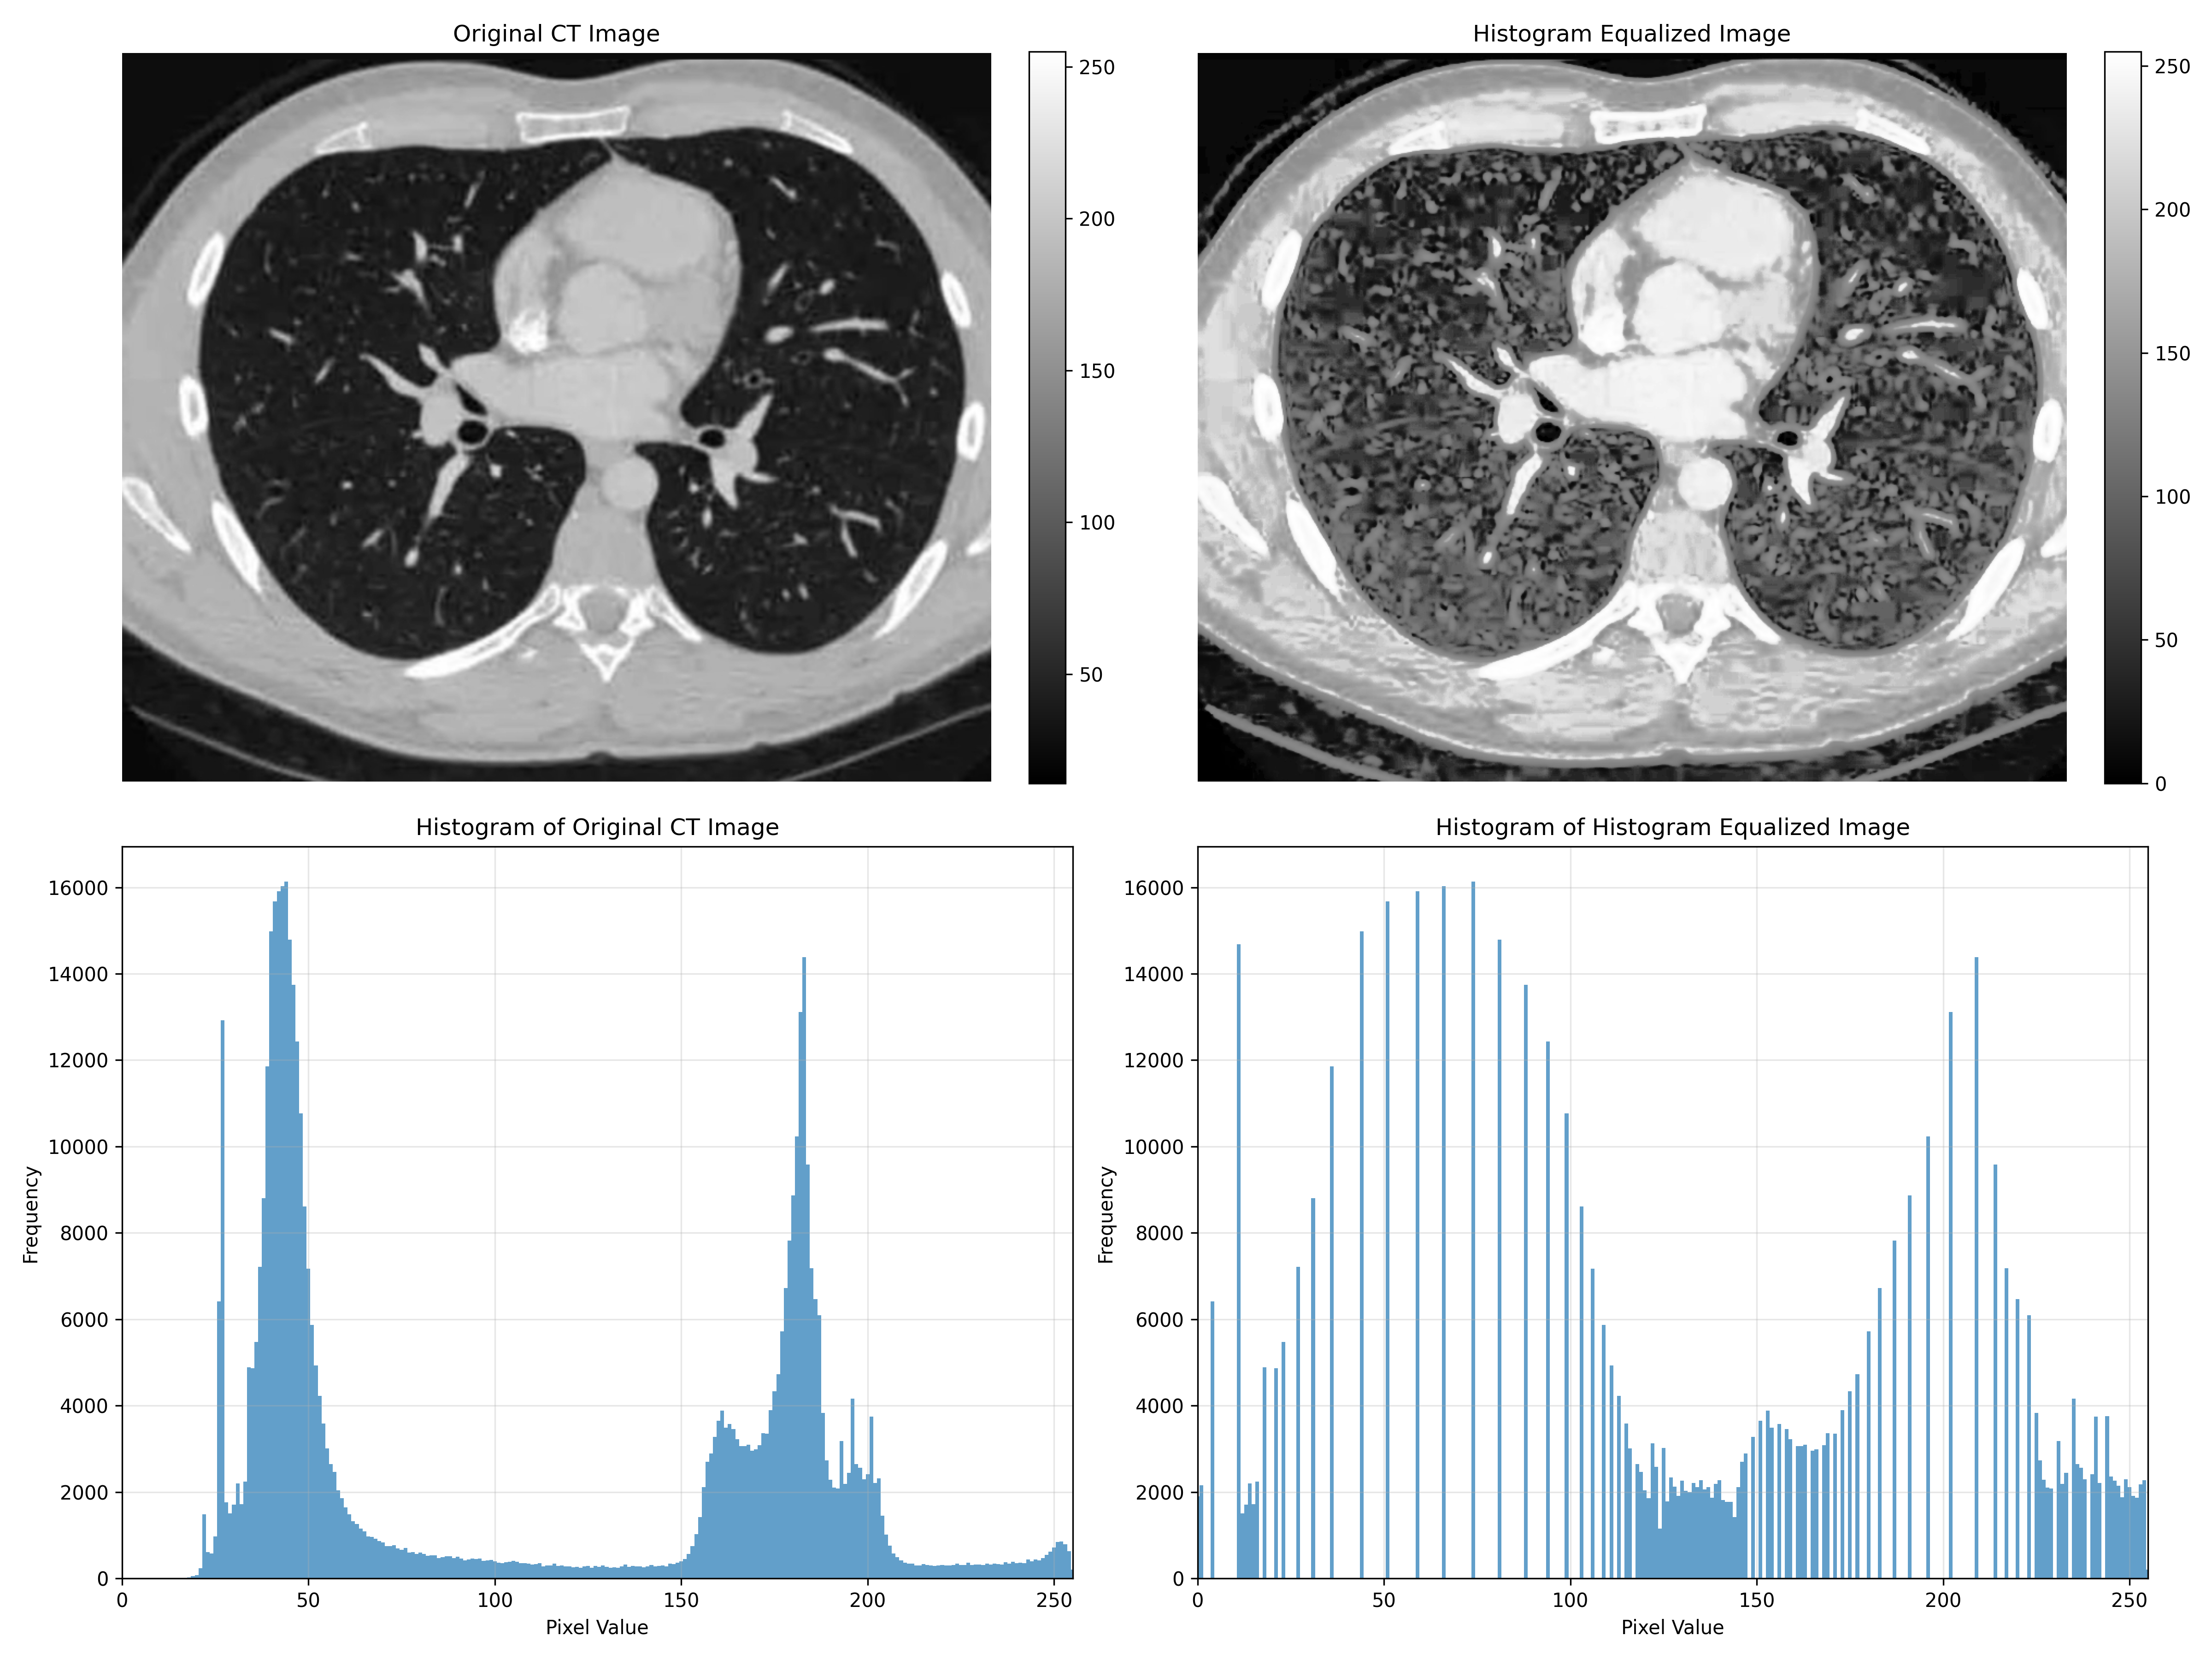
\includegraphics[width=1.0\linewidth]{figures/ct_histogram_equalization.png}
    \caption{CT图像的直方图均衡化结果}
    \label{fig:histogram_eq}
\end{figure}
\begin{figure}[htbp]
    \centering
    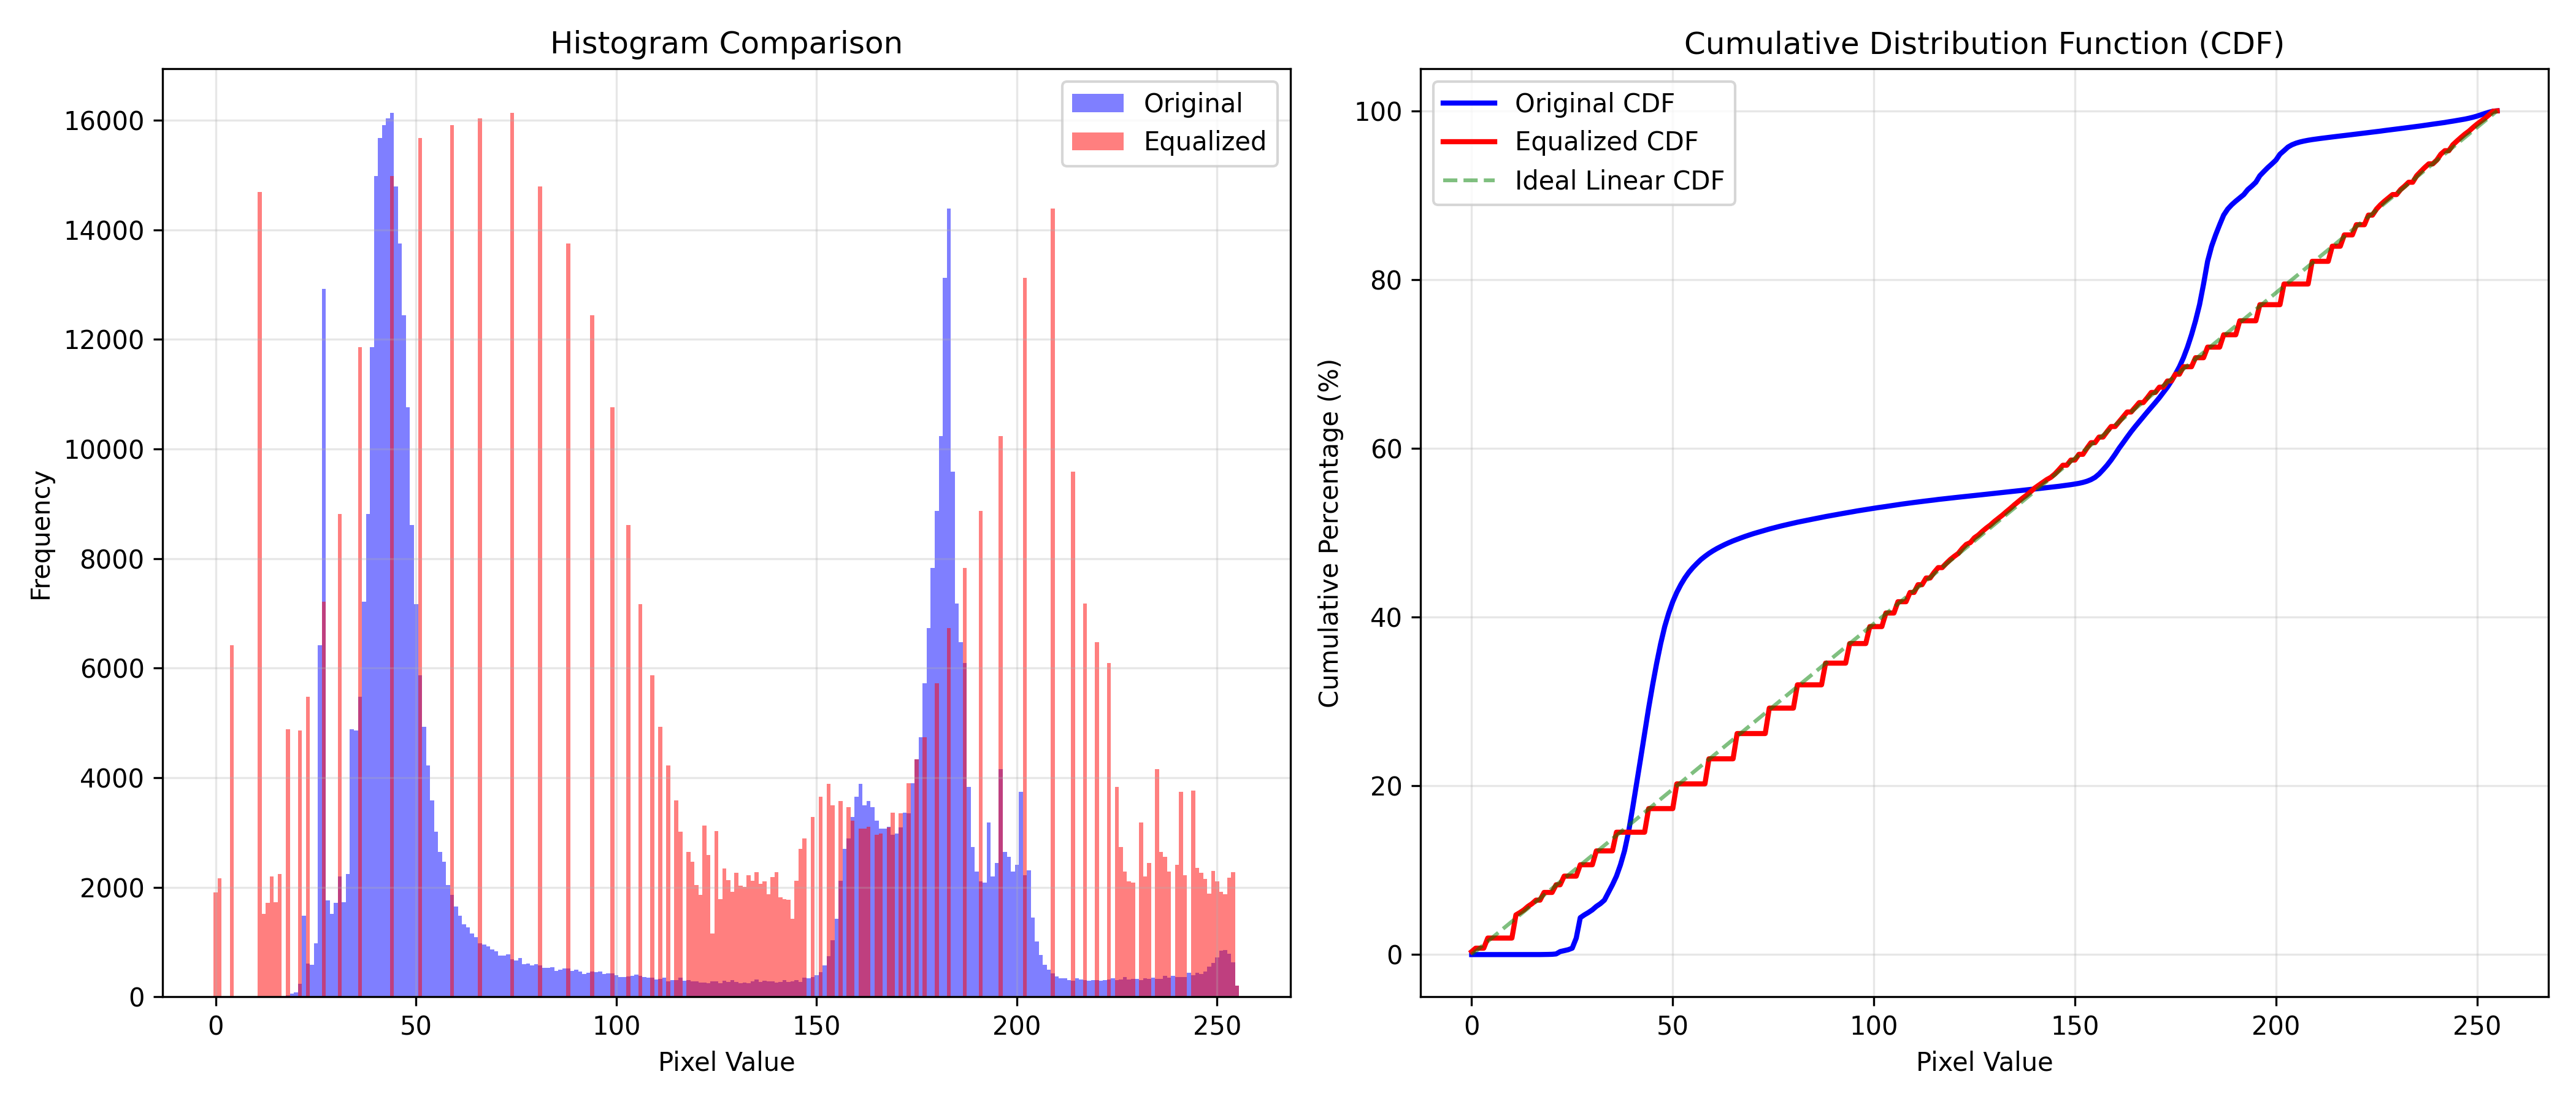
\includegraphics[width=1.0\linewidth]{figures/ct_histogram_cdf_comparison.png}
    \caption{CT图像的直方图均衡化CDF比较}
    \label{fig:histogram_cdf}
\end{figure}
图\ref{fig:histogram_eq}和图\ref{fig:histogram_cdf}展示了CT图像的直方图均衡化结果。左侧为原始图像及其直方图,右侧为均衡化后的图像及其直方图。通过直方图均衡化,原本集中在中低灰度区域的像素值被重新分布到整个灰度范围内,使得图像的对比度显著提高。

从直方图的变化可以看出:
\begin{itemize}
    \item 原始图像的直方图集中在较窄的灰度范围内,而均衡化后的直方图覆盖了更宽的灰度范围
    \item 均衡化后的直方图更加平坦,表明灰度值的分布更加均匀
    \item 原本难以区分的细节在均衡化后变得更加明显,特别是在原本对比度较低的区域
\end{itemize}
\clearpage
\section{讨论、心得}
通过本次实验,我深入了解了医学图像处理的基本技术,包括空间变换、强度变换和直方图处理。对于一些参数选择我发现实际上可以定义一些指标然后自动计算选择得分高的这样会更客观省力。
\end{document}